\section{Results}
\label{sec:results}

We organize results around four questions: Does grounding help overall
(\secref{sec:res-aggregate})? Which mechanism helps, and is it significant
(\secref{sec:res-sig})? How does the answer vary by task
(\secref{sec:res-pertask})? And do novelty, diversity, and cost track usefulness
(\secref{sec:res-novelty})?

\subsection{Grounding does not uniformly help}
\label{sec:res-aggregate}

\tabref{tab:aggregate} reports mean accuracy per regime, averaged over $3$ tasks
$\times\, 3$ seeds. The empirical regime (C3) has the best \IND{} accuracy
($0.676$), and the ungrounded control (C0) has the best \OOD{} accuracy ($0.760$).
Pooling the five grounded regimes against C0 (our H1 test), grounding is
statistically indistinguishable from---and slightly below---the control: \IND{}
$0.619$ vs.\ $0.631$ ($d{=}-0.32$, $p{=}0.37$) and \OOD{} $0.735$ vs.\ $0.760$
($d{=}-0.41$, $p{=}0.25$). The blanket claim ``grounding makes a strong LLM's ideas
better'' is \emph{not} supported.

\begin{table}[t]
\centering
\caption{Aggregate accuracy by regime (mean over $3$ tasks $\times\, 3$ seeds).
\textbf{Best per column in bold.} Grounding does not uniformly beat the ungrounded
control C0: C3 (empirical) is best \IND, but C0 is best \OOD. Diversity is mean
pairwise cosine distance within a bank; novelty distance is mean cosine distance to
the held-out expert hypotheses; generation tokens per bank span $\sim\!80\times$.}
\label{tab:aggregate}
\resizebox{\textwidth}{!}{%
\begin{tabular}{@{}lcccccccr@{}}
\toprule
\textbf{Regime} & \textbf{\IND{} acc} & \textbf{\IND{} sd} & \textbf{\OOD{} acc} & \textbf{\OOD{} sd} & \textbf{Diversity} & \textbf{Novelty} & \textbf{Gen tok/bank} \\
\midrule
C0 \Cungrounded{} (control) & $0.631$ & $.079$ & $\mathbf{0.760}$ & $.183$ & $0.417$ & $0.399$ & $\mathbf{460}$ \\
C1 \Cdeduction{}           & $0.608$ & $.071$ & $0.766$ & $.166$ & $0.367$ & $0.399$ & $918$ \\
C2 \Cinduction{}           & $0.637$ & $.053$ & $0.719$ & $.113$ & $0.409$ & $0.431$ & $2{,}897$ \\
C3 \Cempirical{}           & $\mathbf{0.676}$ & $.095$ & $0.739$ & $.117$ & $0.392$ & $0.430$ & $36{,}935$ \\
C4 \Cliterature{}          & $0.601$ & $.032$ & $0.721$ & $.175$ & $0.396$ & $0.415$ & $1{,}150$ \\
C5 \Cproposal{}            & $0.574$ & $.070$ & $0.729$ & $.183$ & $0.308$ & $0.415$ & $1{,}588$ \\
\bottomrule
\end{tabular}}
\end{table}

\begin{figure}[t]
\centering
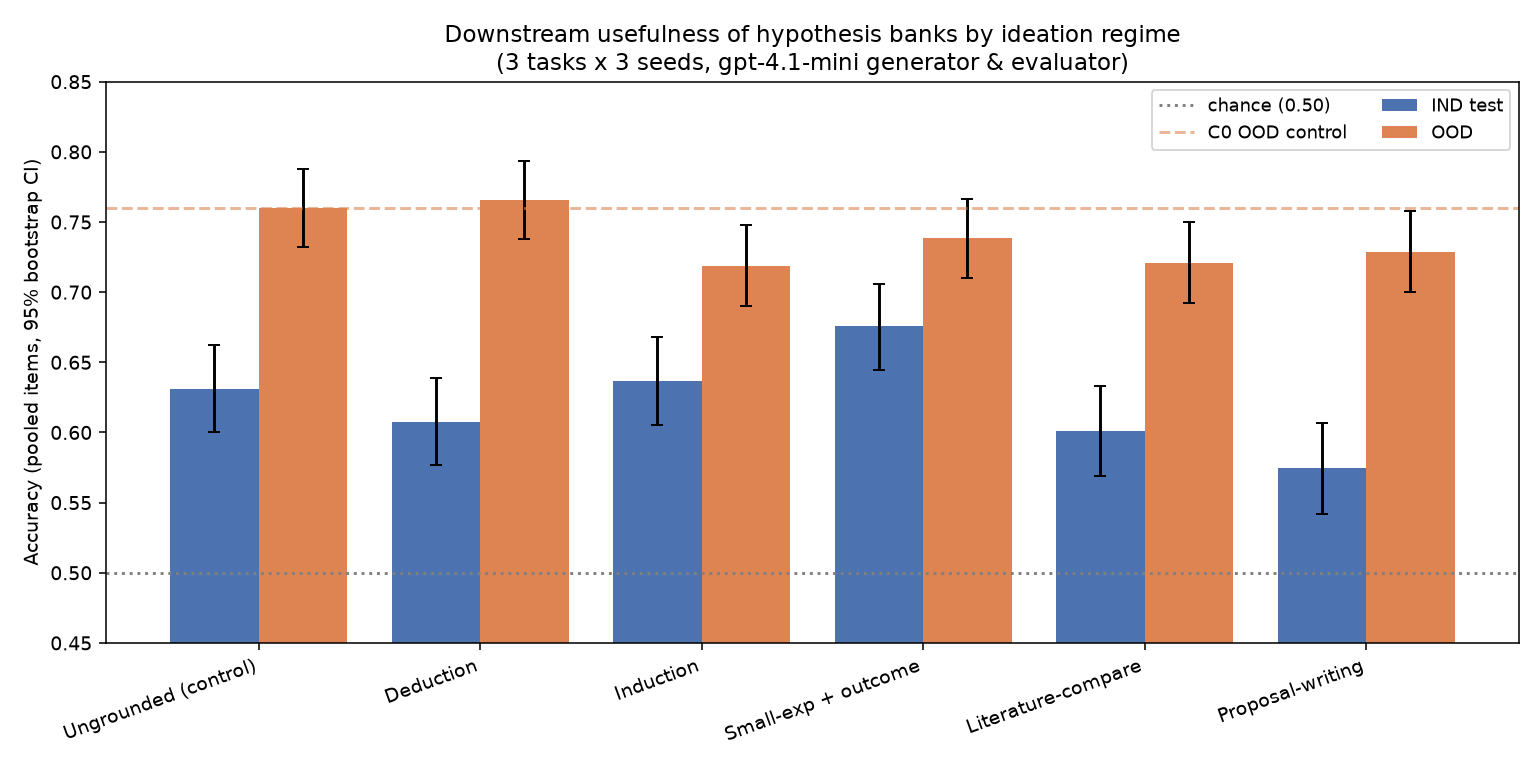
\includegraphics[width=0.95\linewidth]{figures/fig1_accuracy_by_regime.png}
\caption{In-distribution (\IND) and out-of-distribution (\OOD) accuracy by regime,
with bootstrap $95\%$ confidence intervals. The empirical regime (C3) leads
\IND; the ungrounded control (C0) leads \OOD. The chance line is at $0.50$. Mean
differences between most grounded regimes and the control are small relative to the
confidence intervals.}
\label{fig:accuracy}
\end{figure}

\subsection{The mechanism matters: empirical grounding helps, proposal writing hurts}
\label{sec:res-sig}

\tabref{tab:significance} gives the paired comparison of each grounded regime against
the control. Two regimes move the needle, in opposite directions. \Cempirical{} (C3)
is the only regime that \emph{significantly improves} \IND{} accuracy ($+0.044$,
$d{=}1.09$, Wilcoxon $p{=}0.020$); it is the one mechanism that changes its ideas in
response to evidence---it tests the bank, sees concrete mistakes, and revises.
\Cproposal{} (C5) \emph{significantly hurts} \IND{} accuracy ($-0.057$, $d{=}-1.56$,
$p{=}0.008$), surviving the Bonferroni correction, and it has by far the lowest
diversity ($0.308$ in \tabref{tab:aggregate}). The remaining regimes (deduction,
induction, literature comparison) are within noise of the control. No grounded regime
significantly beats the control \OOD. This supports H2 only partially---empirical
grounding leads on \IND, but the full predicted ordering does not hold---and refutes
H3: the grounding advantage is \emph{not} larger \OOD, and is often reversed
(\figref{fig:advantage}).

\begin{table}[t]
\centering
\caption{Paired significance of each grounded regime vs.\ the ungrounded control C0
($9$ paired task$\times$seed cells; Bonferroni $m{=}5$). \textbf{Bold} marks
significant effects ($p<0.05$). Empirical grounding (C3) is the only regime that
significantly improves \IND{} accuracy; proposal writing (C5) significantly hurts and
survives Bonferroni correction. No grounded regime significantly beats C0 \OOD.}
\label{tab:significance}
\resizebox{0.85\textwidth}{!}{%
\begin{tabular}{@{}llcccc@{}}
\toprule
\textbf{Split} & \textbf{Regime} & \textbf{Gain vs.\ C0} & \textbf{Cohen's $d$} & \textbf{Wilcoxon $p$} & \textbf{$t$ $p$ (Bonf.)} \\
\midrule
\IND{} & C1 \Cdeduction{}   & $-0.023$ & $-0.51$ & $0.195$ & $0.826$ \\
\IND{} & C2 \Cinduction{}   & $+0.006$ & $+0.11$ & $0.785$ & $1.000$ \\
\IND{} & \textbf{C3 \Cempirical{}} & $\mathbf{+0.044}$ & $\mathbf{+1.09}$ & $\mathbf{0.020}$ & $0.058$ \\
\IND{} & C4 \Cliterature{}  & $-0.030$ & $-0.46$ & $0.195$ & $1.000$ \\
\IND{} & \textbf{C5 \Cproposal{}} & $\mathbf{-0.057}$ & $\mathbf{-1.56}$ & $\mathbf{0.008}$ & $\mathbf{0.008}$ \\
\midrule
\OOD{} & C1 \Cdeduction{}   & $+0.006$ & $+0.14$ & $0.719$ & $1.000$ \\
\OOD{} & C2 \Cinduction{}   & $-0.041$ & $-0.29$ & $0.652$ & $1.000$ \\
\OOD{} & C3 \Cempirical{}   & $-0.021$ & $-0.19$ & $0.742$ & $1.000$ \\
\OOD{} & C4 \Cliterature{}  & $-0.039$ & $-0.54$ & $0.102$ & $0.715$ \\
\OOD{} & C5 \Cproposal{}    & $-0.031$ & $-0.47$ & $0.234$ & $0.988$ \\
\bottomrule
\end{tabular}}
\end{table}

\begin{figure}[t]
\centering
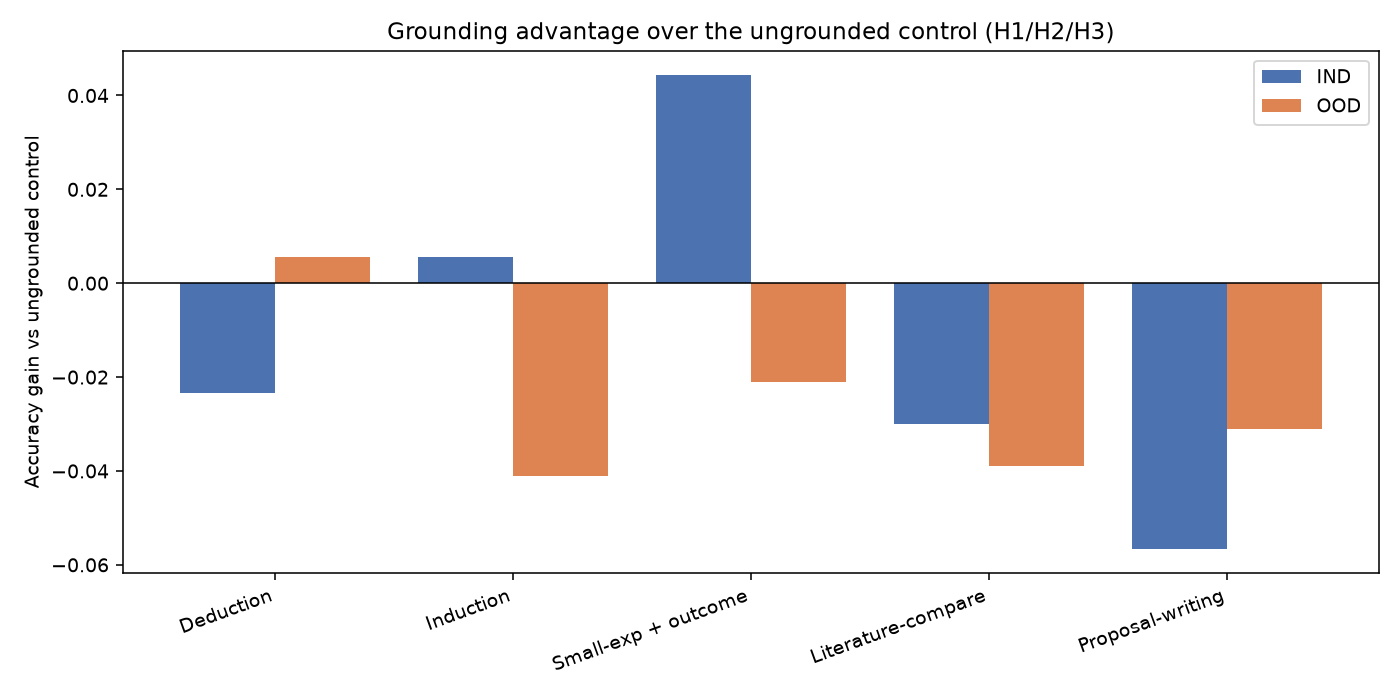
\includegraphics[width=0.7\linewidth]{figures/fig2_grounding_advantage.png}
\caption{Grounding advantage (regime accuracy minus control C0) on \IND{} and \OOD.
Only empirical grounding (C3) shows a clear positive \IND{} advantage; proposal
writing (C5) shows a clear negative one. Contrary to H3, advantages are not larger
\OOD---the \OOD{} bars are mostly negative.}
\label{fig:advantage}
\end{figure}

\subsection{Three tasks, three stories: heterogeneity and overfitting}
\label{sec:res-pertask}

The aggregate masks sharp per-task heterogeneity (\tabref{tab:pertask},
\figref{fig:heatmap}). On \dreaddit, empirical grounding (C3) wins clearly on
\emph{both} \IND{} ($0.78$ vs.\ $0.72$) and \OOD{} ($0.81$ vs.\ $0.75$)---here
grounding genuinely helps. On \deceptive, the ungrounded model transfers
near-perfectly \OOD{} ($0.97$) using general priors, while data grounding (C2/C3)
\emph{raises} \IND{} but \emph{crashes} \OOD{} to $0.78$--$0.82$: the learned rules
encode dataset-specific surface cues (\eg spatial/Chicago-hotel vocabulary) that do
not transfer, whereas the ungrounded prior captures general ``fake review'' structure
that does. This is the paper's most important nuance: \emph{data grounding can overfit},
trading \OOD{} robustness for \IND{} fit---a caution prior work, which emphasizes data
grounding's \OOD{} \emph{wins}, under-reports. On \headline, all regimes hover near
chance ($0.50$--$0.61$), including the expert hypotheses ($0.56/0.58$); there is little
extractable signal, so the task contributes mostly noise to the aggregate.

\begin{table}[t]
\centering
\caption{Per-task accuracy (\IND{} / \OOD, mean over seeds) for selected regimes.
\textbf{Bold} marks the best \IND/\OOD{} on a task among the shown regimes. Three
distinct stories: grounding helps on \dreaddit, overfits on \deceptive{} (ungrounded
\OOD{} $0.97$ vs.\ grounded $\le 0.82$), and finds no signal on \headline.}
\label{tab:pertask}
\resizebox{0.8\textwidth}{!}{%
\begin{tabular}{@{}lccc@{}}
\toprule
\textbf{Regime} & \textbf{\headline} & \textbf{\deceptive} & \textbf{\dreaddit} \\
\midrule
C0 \Cungrounded{} & $0.55 / 0.56$ & $0.62 / \mathbf{0.97}$ & $0.72 / 0.75$ \\
C2 \Cinduction{}  & $0.58 / 0.61$ & $0.65 / 0.78$ & $0.68 / 0.77$ \\
C3 \Cempirical{}  & $0.56 / 0.59$ & $\mathbf{0.69} / 0.82$ & $\mathbf{0.78} / \mathbf{0.81}$ \\
C5 \Cproposal{}   & $0.50 / 0.57$ & $0.58 / 0.97$ & $0.64 / 0.65$ \\
\bottomrule
\end{tabular}}
\end{table}

\begin{figure}[t]
\centering
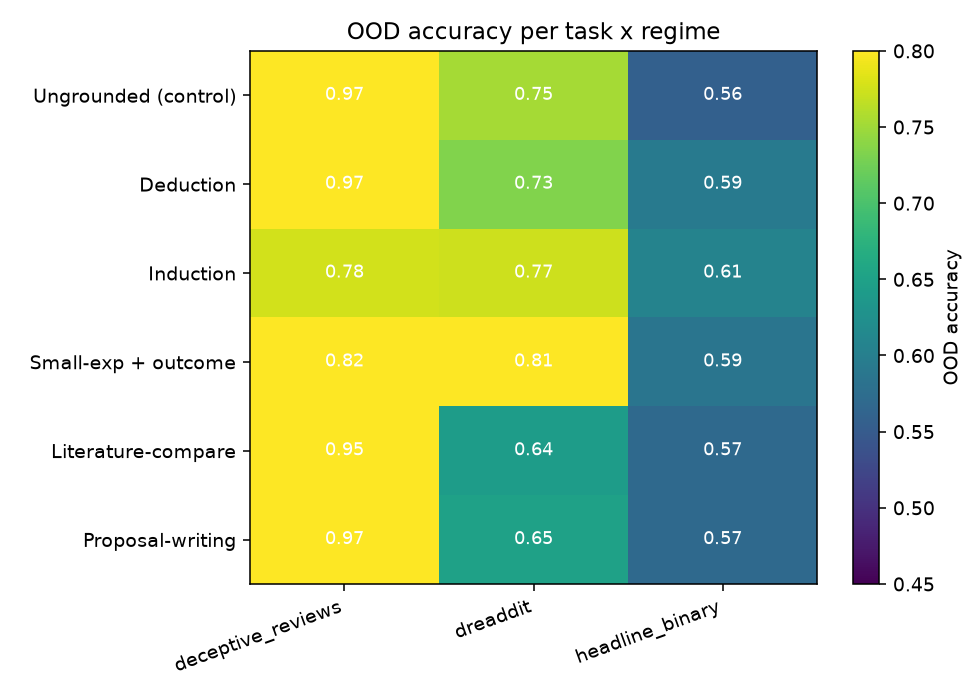
\includegraphics[width=0.95\linewidth]{figures/fig5_per_task_heatmap.png}
\caption{Per-task accuracy grid across all six regimes (\IND{} and \OOD).
The heterogeneity is stark: \dreaddit{} rewards grounding, \deceptive{} shows the
ungrounded control's near-perfect \OOD{} transfer collapsing under data grounding,
and \headline{} sits near chance throughout.}
\label{fig:heatmap}
\end{figure}

\subsection{Cost, novelty, and diversity do not buy usefulness}
\label{sec:res-novelty}

\para{Cost/benefit.} C3's \IND{} gain is expensive: it costs $\sim\!80\times$ the
generation tokens of the control ($36.9$k vs.\ $0.46$k tokens/bank), driven by its
test-and-revise loop (\figref{fig:cost}). The cheaper grounded regimes (C1, C4, C5 at
$0.9$k--$1.6$k tokens) do \emph{not} beat the control. Grounding's one reliable win
comes only at the top of the cost curve.

\para{Novelty $\neq$ usefulness.} Across the $18$ task$\times$regime cells,
Spearman$(\text{novelty},\,\OOD)=+0.835$ ($p<0.001$)---but this is a task-difficulty
confound (a Simpson's paradox): easy, high-accuracy tasks also have ideas farther from
their expert anchors. \emph{Within} a task the relationship vanishes (mean
$\rho\approx-0.10$; \deceptive{} $\rho=-0.75$), and diversity$\to$usefulness is weak
within task (mean $\rho\approx+0.33$, n.s.). Novelty and diversity are therefore not
reliable proxies for usefulness (\figref{fig:novelty}), consistent with the
literature's caveat and confirming H4 once the task confound is removed.

\begin{figure}[t]
\centering
\begin{subfigure}[b]{0.48\textwidth}
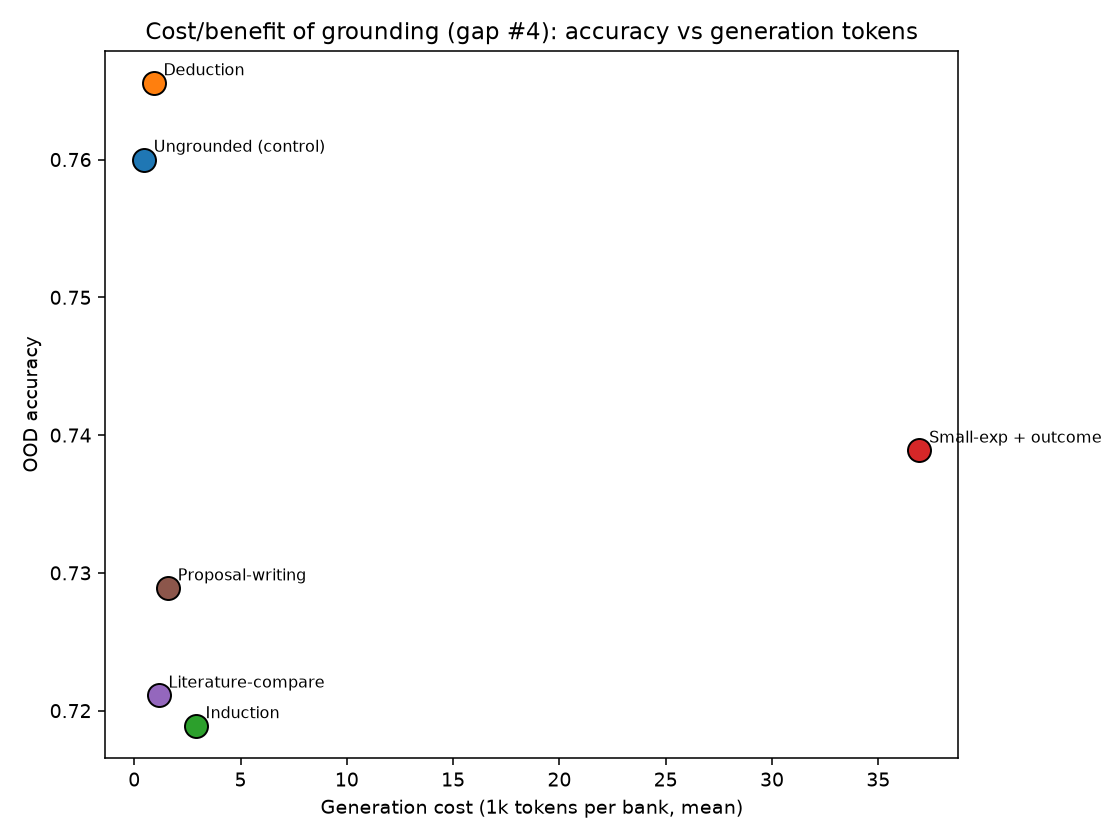
\includegraphics[width=\textwidth]{figures/fig4_cost_benefit.png}
\caption{Cost vs.\ benefit}
\label{fig:cost}
\end{subfigure}
\hfill
\begin{subfigure}[b]{0.48\textwidth}
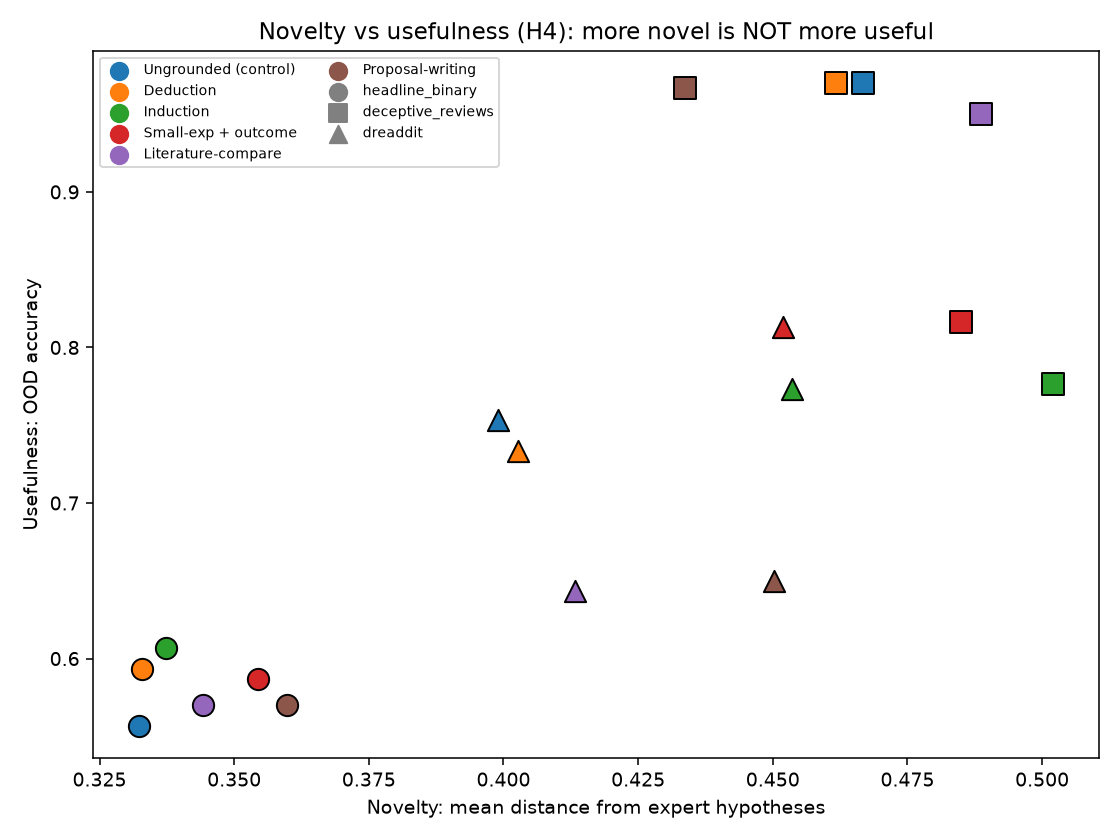
\includegraphics[width=\textwidth]{figures/fig3_novelty_vs_usefulness.png}
\caption{Novelty vs.\ usefulness}
\label{fig:novelty}
\end{subfigure}
\caption{\captiona{} \figleft{} Generation tokens per bank vs.\ \IND{} accuracy:
empirical grounding (C3) buys its gain at $\sim\!80\times$ the control's token cost,
while cheaper grounded regimes do not beat the control. \captionb{} \figright{} Bank
novelty (distance from expert hypotheses) vs.\ \OOD{} usefulness: the strong pooled
correlation is a task-difficulty confound that vanishes within task, so novelty does
not track usefulness.}
\label{fig:costnovelty}
\end{figure}
